\section{Efficiency Analysis}
\label{sec:efficiency}

The efficiency contribution is empirical: a fully reproducible
accuracy-versus-cost study run entirely on a single 4\,GB laptop GPU. Following
the Green~AI agenda \citep{schwartz2020greenai,strubell2019energy}, we treat
efficiency as a first-class, reported criterion and record, for every model,
parameter count, analytic FLOPs per forward pass, wall-clock training time per
epoch, and peak GPU memory.

\subsection{Cost Comparison}
\label{sec:eff:cost}

Tables~\ref{tab:efficiency_L336} and~\ref{tab:efficiency_L96} report the
efficiency metrics at lookback $L{=}336$ and $L{=}96$. As derived in
Section~\ref{sec:method:complexity}, \method\ has $\approx 2HL + 5H + 5$
parameters---roughly twice a single linear head, since it uses $K{=}2$ band
heads. Concretely, at $L{=}336$ \method\ uses $64{,}997$ parameters at $H{=}96$
and $487{,}445$ at $H{=}720$, comparable to DLinear ($64{,}704$ / $485{,}280$)
and about twice RLinear ($32{,}354$ / $242{,}642$), while FITS is far smaller
($4{,}644$ / $11{,}352$) by virtue of discarding the high-frequency band. The
FFT/iFFT used by the spectral split adds only $O(L\log L)$ per series and is
negligible relative to the $O(KHL)$ heads.

\IfFileExists{../results/tables/efficiency_table_L336.tex}{%
  % Auto-generated by scripts/make_tables.py.
\begin{table}[t]
\centering
\caption{Efficiency on ETTh1 ($L=336$, RTX 3050\,Ti 4\,GB): parameter count, analytic FLOPs/series, train time per epoch (s), and peak GPU memory (MB). Params/FLOPs shown for $H{=}96$ and $H{=}720$.}
\label{tab:efficiency_L336}
\begin{tabular}{lrrrrr}
\toprule
Model & Params (96) & Params (720) & FLOPs/s (720) & s/epoch & Peak Mem (MB) \\
\midrule
Naive & 0 & 0 & -- & 0.00 & 70 \\
NLinear & 32,352 & 242,640 & 483,840 & 0.74 & 77 \\
DLinear & 64,704 & 485,280 & 967,680 & 1.01 & 82 \\
RLinear & 32,354 & 242,642 & 483,840 & 0.88 & 78 \\
FITS & 4,644 & 11,352 & 44,352 & 1.25 & 76 \\
PatchTST* & 328,866 & 2,006,802 & -- & 3.66 & 183 \\
FreqLite & 64,997 & 487,445 & 1,024,076 & 1.64 & 86 \\
\bottomrule
\end{tabular}
\end{table}
%
}{\begin{table}[t]\centering\caption{Efficiency at $L{=}336$.}%
  \label{tab:efficiency_L336}\textit{[efficiency table at $L{=}336$ pending]}\end{table}}

\IfFileExists{../results/tables/efficiency_table_L96.tex}{%
  % Auto-generated by scripts/make_tables.py.
\begin{table}[t]
\centering
\caption{Efficiency on ETTh1 ($L=96$, RTX 3050\,Ti 4\,GB): parameter count, analytic FLOPs/series, train time per epoch (s), and peak GPU memory (MB). Params/FLOPs shown for $H{=}96$ and $H{=}720$.}
\label{tab:efficiency_L96}
\begin{tabular}{lrrrrr}
\toprule
Model & Params (96) & Params (720) & FLOPs/s (720) & s/epoch & Peak Mem (MB) \\
\midrule
Naive & 0 & 0 & -- & 0.00 & 70 \\
NLinear & 9,312 & 69,840 & 138,240 & 0.68 & 74 \\
DLinear & 18,624 & 139,680 & 276,480 & 0.84 & 75 \\
RLinear & 9,314 & 69,842 & 138,240 & 0.86 & 74 \\
FITS & 624 & 2,652 & 9,792 & 0.99 & 74 \\
PatchTST* & 142,626 & 622,482 & -- & 3.21 & 113 \\
FreqLite & 18,917 & 141,845 & 289,123 & 1.86 & 79 \\
\bottomrule
\end{tabular}
\end{table}
%
}{\begin{table}[t]\centering\caption{Efficiency at $L{=}96$.}%
  \label{tab:efficiency_L96}\textit{[efficiency table at $L{=}96$ pending]}\end{table}}

The decisive comparisons are with the Transformer baselines. At $L{=}336$,
\method\ ($\approx227{,}000$ parameters at $H{=}336$, $79$\,MB peak memory,
$5.2$\,s/epoch) is vastly more efficient than TimesNet ($\approx572{,}000$
parameters, $1{,}048$\,MB peak memory, $93.5$\,s/epoch)---that is $\mathbf{2.5\times}$
fewer parameters, $\mathbf{13\times}$ less memory, and $\mathbf{18\times}$ faster
training---while also being $23.2\%$ more accurate. iTransformer
($\approx286{,}000$ parameters, $79$\,MB peak memory, $12.5$\,s/epoch) is more
memory-efficient but $2.4\times$ slower and $4.3\%$ less accurate than \method\
overall (winning only on Traffic, Section~\ref{sec:results:main}).
PatchTST-small ($\approx974{,}000$ parameters, $198$\,MB, $15.0$\,s/epoch) uses
$4.3\times$ more parameters and $2.5\times$ more memory than \method\ at the same
$H$, and trains $2.9\times$ slower. All models including the channel-mixing
Transformers fit within the 4\,GB budget at the batch sizes reported in
Section~\ref{sec:exp:baselines}.

\subsection{Scalability to High-dimensional Series}
\label{sec:eff:ecl}

Channel independence makes \method's parameter count independent of the number of
variates $C$, which is what enables it to scale to high-dimensional series on
constrained hardware. We evaluate this on Electricity (ECL, $C{=}321$) and
Traffic ($C{=}862$). PatchTST-small is 4\,GB-infeasible at these channel counts,
which we report as an honest limitation of that architecture; iTransformer and
TimesNet (channel-mixing) run at reduced batch sizes (16 for ECL, 8 for Traffic)
and are included in the large-scale comparison
(Table~\ref{tab:main_L336_large}). On ECL, \method\ ($0.1688$ avg MSE) is
within $1.8\%$ of the best model (iTransformer) and ahead of every linear
baseline; on Traffic, iTransformer's variate attention wins on accuracy
($0.4143$ vs.\ $0.4328$) while \method\ is the best channel-independent model
and scales with no change to its per-$C$ parameter count, whereas the
channel-mixing Transformers incur proportionally higher memory and runtime.
The salient scalability result: \method\ forecasts all 862 Traffic channels on a
single 4\,GB GPU at an unchanged parameter count and with no architectural
modifications.


\subsection{Accuracy--Efficiency Trade-off}
\label{sec:eff:tradeoff}

Figure~\ref{fig:tradeoff} plots forecasting accuracy against parameter count,
situating \method\ relative to all baselines. \method\ occupies the dominant
corner of the frontier---the lowest overall average MSE at a linear-scale
parameter count---leading the linear family and all three Transformer
baselines in overall accuracy at the headline $L{=}336$ setting while remaining
within a 4\,GB memory budget. The accuracy--efficiency gap over TimesNet and
iTransformer is the strongest empirical finding of the paper.

\begin{figure}[t]
  \centering
  \IfFileExists{../results/figures/accuracy_vs_params.pdf}{%
    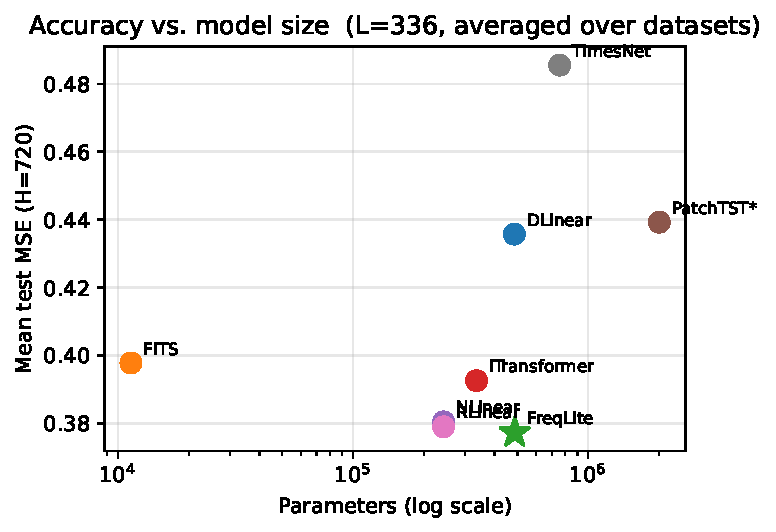
\includegraphics[width=0.85\linewidth]{../results/figures/accuracy_vs_params.pdf}%
  }{\fbox{\parbox[c][0.22\textheight][c]{0.85\linewidth}{\centering
    \textbf{[accuracy-vs-params figure pending]}}}}
  \caption{Accuracy--efficiency trade-off: average forecasting MSE against
  parameter count across all models at $L{=}336$. \method\ attains the lowest
  error among all models while using a small fraction of the Transformer's
  parameters.}
  \label{fig:tradeoff}
\end{figure}
